In this section, we will present the execution time of the basic ROMC
functionalities. Apart from performing the inference accurately, one
of the notable advantages of ROMC is its efficiency. In terms of
performance, ROMC holds two key advantages.

Firstly, all its subparts are parallelisable; optimising the objective
functions, constructing the bounding boxes, fitting the local
surrogate models, sampling and evaluating the posterior can be
executed in a fully-parallel fashion. Therefore, the speed-up can be
extended as much as the computational resources allow. Specifically,
at the CPU level, the parallelisation can be incorporate all available
cores. A similar design can be utilised in the case of having a
cluster of PCs available. Parallelising the process at the GPU level
is not that trivial, since the parallel tasks are more complicated
than simple floating-point operations. Our current implementation
supports parallelisation only at the CPU level, exploiting all the cores of the CPU.\footnote{At a future update, it is possible to support parallelising the processes using a cluster of PCs.}. In subsection
\ref{subsubsec:parallel}, we will demonstrate the speed-up achieved
through parallelisation.

The second important advantage concerns the execution of the
training and the inference phase in distinct time-slots. Therefore, one
can consume a lot of training time and resources but ask for
accelerated inference. The use of a lightweight surrogate model around
the optimal point exploits this essential characteristic; it trades
some additional computational burden at the training phase, for
exercising faster inference later. In figures \ref{fig:exec_solve},
\ref{fig:exec_regions}, \ref{fig:exec_posterior},
\ref{fig:exec_sample} we can observe this advantage. The
example measured in these figures is the simple 1D example, used in
the previous chapter. We observe that fitting local surrogate models
slows down the training phase (estimating the regions) by a factor of
$1.5$, but provides a speed-up of $15$ at the inference phase i.e.\
approximating unnormalised posterior. This outcome would be even more
potent in larger models, where running the simulator is even more
expensive.


\begin{figure}[ht]
    \begin{center}
      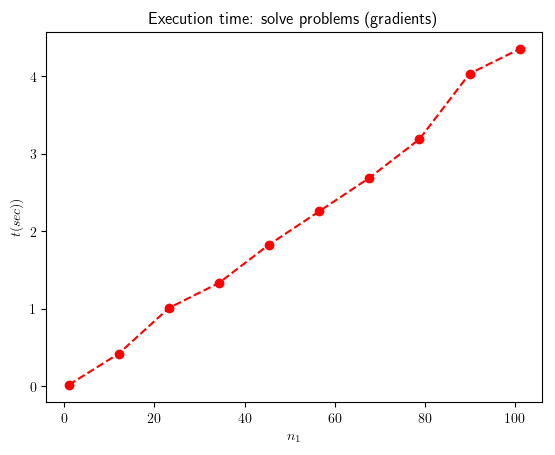
\includegraphics[width=0.48\textwidth]{./Thesis/images/chapter4/exec_solve_grad.png}
      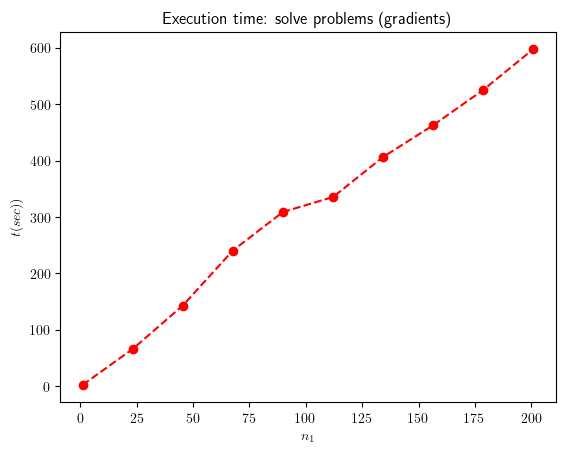
\includegraphics[width=0.48\textwidth]{./Thesis/images/chapter4/exec_solve_bo.png}
    \end{center}
    \caption[Execution time for solving the optimisation problems.]{Execution time for defining and solving the optimisation
      problems. We observe that the Bayesian optimisation scheme is much more expensive, performing the task slower by a factor of $75$.}
  \label{fig:exec_solve}
\end{figure}

\begin{figure}[ht]
    \begin{center}
      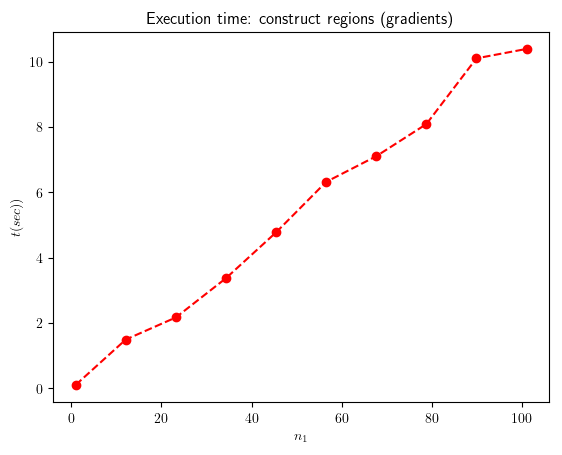
\includegraphics[width=0.48\textwidth]{./Thesis/images/chapter4/exec_regions_grad.png}
      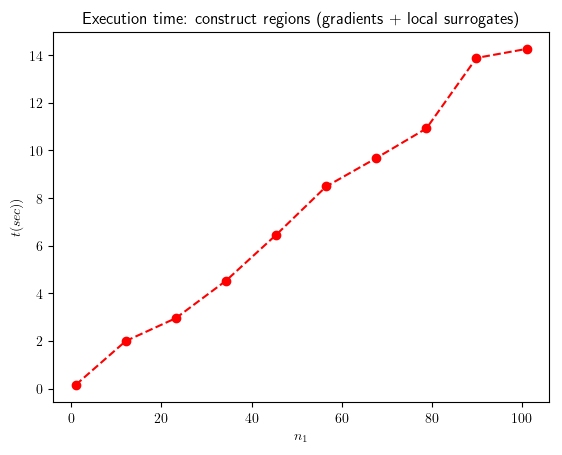
\includegraphics[width=0.48\textwidth]{./Thesis/images/chapter4/exec_regions_grad_fit.png}\\
      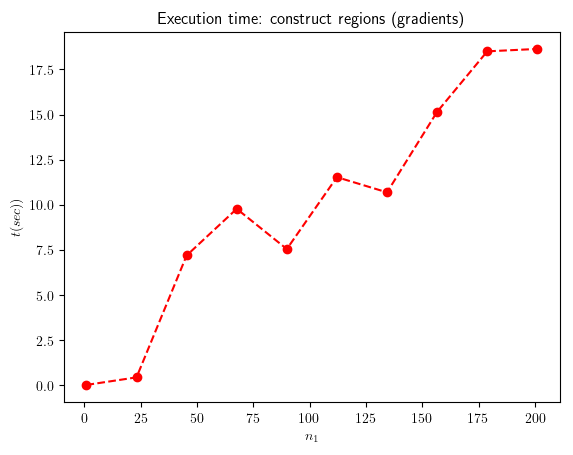
\includegraphics[width=0.48\textwidth]{./Thesis/images/chapter4/exec_regions_bo.png}
      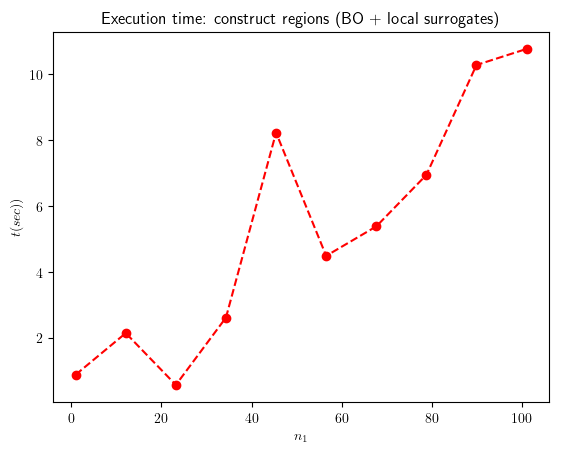
\includegraphics[width=0.48\textwidth]{./Thesis/images/chapter4/exec_regions_bo_fit.png}
    \end{center}
    \caption[Execution time for constructing the n-dimensional bounding box regions.]{Execution time for constructing the n-dimensional
      bounding box region and, optionally, fitting the local surrogate
      models. We observe that fitting the surrogate models incurs a
      small increase by a factor of $1.5$.}
  \label{fig:exec_regions}
\end{figure}


\begin{figure}[ht]
    \begin{center}
      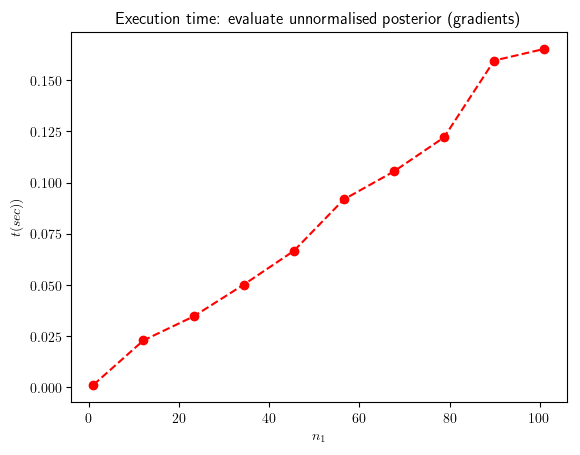
\includegraphics[width=0.48\textwidth]{./Thesis/images/chapter4/exec_posterior_grad.png}
      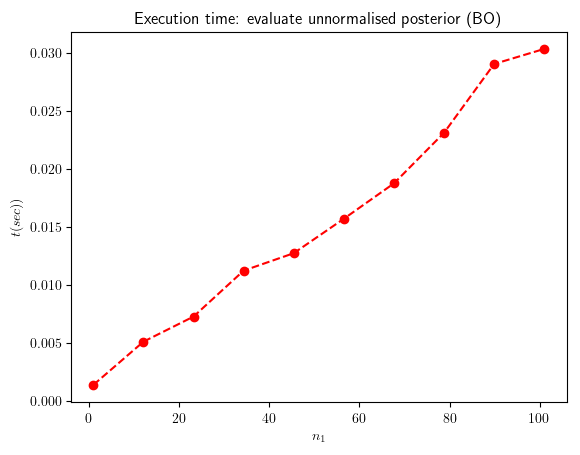
\includegraphics[width=0.48\textwidth]{./Thesis/images/chapter4/exec_posterior_bo.png}\\
      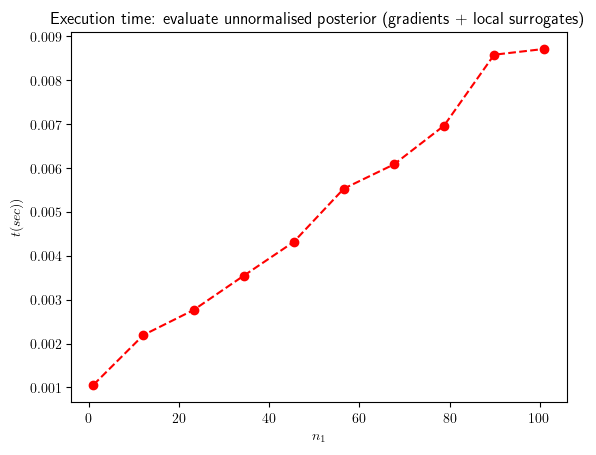
\includegraphics[width=0.48\textwidth]{./Thesis/images/chapter4/exec_posterior_grad_fit.png}
    \end{center}
    \caption[Execution time for evaluation the unnormalised posterior.]{Execution time for evaluating the unnormalised posterior
      approximation. We observe that using a Gaussian Process surrogate model is almost 5 times faster than the simulator and the quadratic local surrogate model 15 times faster.}
  \label{fig:exec_posterior}
\end{figure}


\begin{figure}[ht]
    \begin{center}
      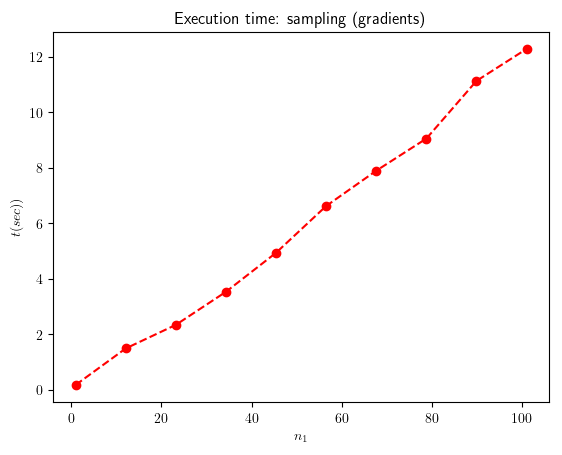
\includegraphics[width=0.48\textwidth]{./Thesis/images/chapter4/exec_sample_grad.png}
      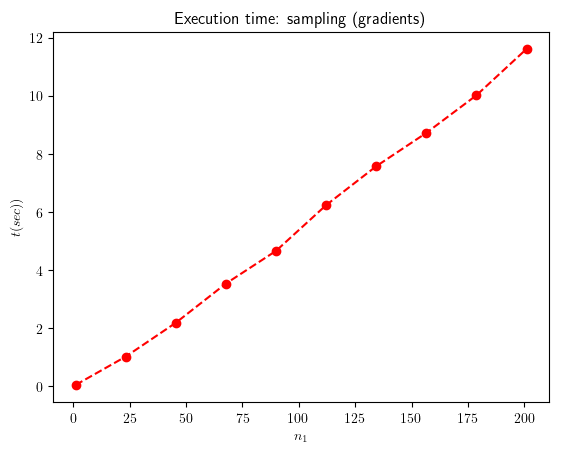
\includegraphics[width=0.48\textwidth]{./Thesis/images/chapter4/exec_sample_bo.png}\\
      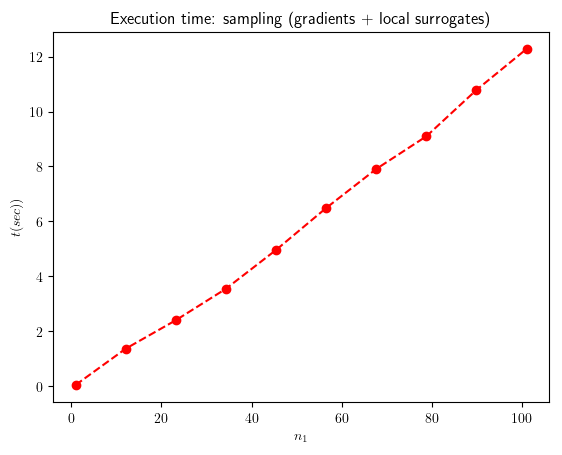
\includegraphics[width=0.48\textwidth]{./Thesis/images/chapter4/exec_sample_grad_fit.png}
    \end{center}
    \caption[Execution time for sampling from the approximate posterior.]{Execution time for sampling from the approximate
      posterior. We observe a small speed-up using the local surrogate model.}
  \label{fig:exec_sample}
\end{figure}

\subsubsection{The effect of parallelisation} \label{subsubsec:parallel}

In this section, we measure the execution times for (a) solving the optimisation problems, (b) construct the bounding boxes, (c) sample from the posterior and (d) evaluate the approximate posterior using parallelisation. The model used for this experiment is the simple two-dimensional example of section \ref{subsec:ex1}. All experiments
have been executed in a laptop Dell XPS 15 with an 8-core CPU. Therefore the maximum expected speed-up can reach a factor of 8. Normally the observed speed-up is lower due to the overhead of setting-up the parallel processes. The experiments confirm our general expectation; the parallel version performs all tasks between 2.5 and 6 times faster compared to the sequential, as shown in figures \ref{fig:exec_parallel} and \ref{fig:exec_parallel2}. The most benefited task is solving the optimisation problems which is performed almost 6 times faster. Sampling is executed 3.5 times faster, whereas evaluating the posterior and constructing the bounding boxes almost 2.5 times faster. 

\begin{figure}[ht]
    \begin{center}
      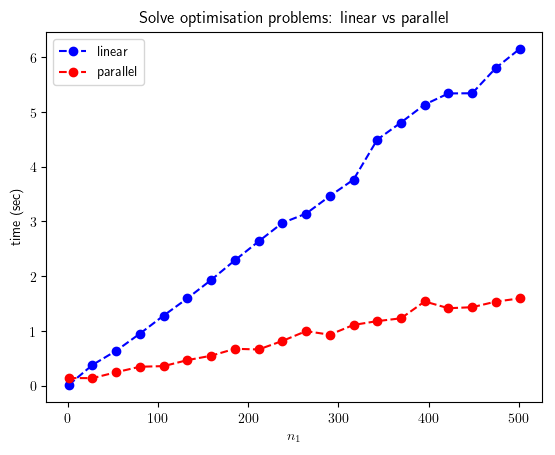
\includegraphics[width=0.48\textwidth]{./Thesis/images/chapter4/solve_problems_parallel.png}
      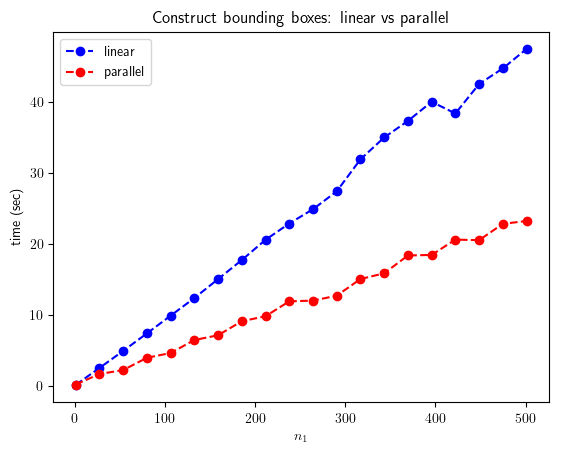
\includegraphics[width=0.48\textwidth]{./Thesis/images/chapter4/estimate_regions_parallel.png}
    \end{center}
    \caption[Execution time of the training part exploiting parallelisation]{Execution
      time of the training part exploiting parallelisation. At the left figure, we measure
      the execution time for solving the optimisation problems. At the
      right figure, we measure the execution time for constructing the
      bounding boxes.}
  \label{fig:exec_parallel}
\end{figure}

\begin{figure}[ht]
    \begin{center}
      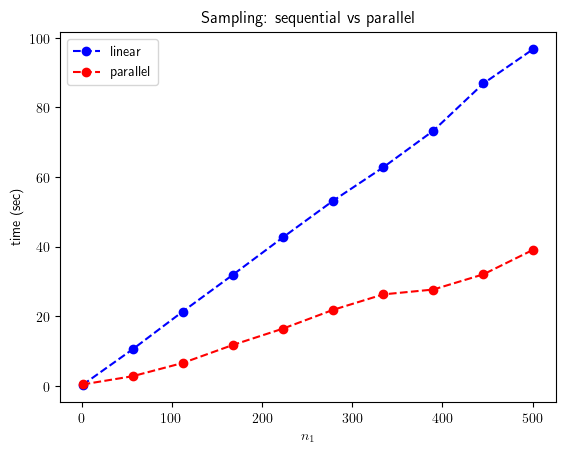
\includegraphics[width=0.48\textwidth]{./Thesis/images/chapter4/sample_parallel.png}
      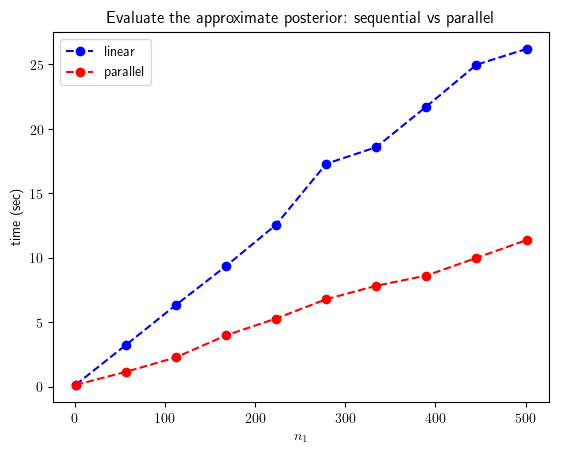
\includegraphics[width=0.48\textwidth]{./Thesis/images/chapter4/eval_post_parallel.png}
    \end{center}
    \caption[Execution time of the inference part exploiting parallelisation.]{Execution
      time of the inference part exploiting parallelisation. At the left figure, we measure
      the execution time for sampling $n_2=50$ points per region. At the right figure we measure the execution time for evaluating the posterior at a batch of $50$ points.}
  \label{fig:exec_parallel2}
\end{figure}